\documentclass[notes,blackandwhite,mathsans,usenames,dvipsnames]{beamer}

\usepackage{amsmath}
\usepackage{amssymb}
\usepackage{graphicx}
\usepackage{fancybox}
\usepackage{booktabs}
\usepackage{multirow,multicol,pxfonts}
\usepackage{cmbright}
\usepackage{xcolor}
\usepackage{color}
\usepackage{enumitem}
\usepackage{animate}
\usepackage{changepage}

\usepackage[T1]{fontenc}
\fontencoding{T1}  
\usepackage[utf8]{inputenc}


\usefonttheme{default}
\setbeamercovered{invisible}
\beamertemplatenavigationsymbolsempty

\makeatletter
\setbeamertemplate{footline}
{
  \leavevmode
  \hbox{
  \begin{beamercolorbox}[wd=0.97\paperwidth,ht=2.25ex,dp=2ex,right]{}
{\color{gre} \insertframenumber{} / \inserttotalframenumber}
  \end{beamercolorbox}}%
}




\definecolor{yel}{HTML}{FED500}
\definecolor{gre}{HTML}{4EB1AD}
\definecolor{blu}{HTML}{865BB8}

\setbeamercolor{frametitle}{fg=gre}
\AtBeginDocument{\color{blu}}
\setbeamertemplate{itemize item}[triangle]




\begin{document}
%\fontfamily{pag}\selectfont
%\setbeamerfont{title}{family=\fontfamily{pag}\selectfont}
%\setbeamerfont{frametitle}{family=\fontfamily{pag}\selectfont}
%\setbeamerfont{framesubtitle}{family=\fontfamily{pag}\selectfont}







{\setbeamercolor{background canvas}{bg=gre}
\begin{frame}

\vspace{1cm}
\begin{tabular}{rl}
&\textbf{\LARGE\color{yel} Macroeconometrics}\\[8ex]
\textbf{\large\color{yel} Lecture 22}&\textbf{\large\color{blu}Less than $\mathbf{2^{\circ}}$C warming by 2100 unlikely}\\[7ex]
&{\large\color{white} Topics in Climate Change}\\
&{\large\color{white} Forecasting CO$_2$ Emissions for the 21st Century}\\[7ex]
&\textbf{Tomasz Wo\'zniak}\\[2ex]
%&\colorbox{blu}{\textit{\small\color{white}\href{https://www.schoolstrike4climate.com/may21}{\#CLIMATESTRIKE MAY21}}}
%&{\small\color{white} Department of Economics}\\
%&{\small\color{white}University of Melbourne}
\end{tabular}

\end{frame}
}



{\setbeamercolor{background canvas}{bg=gre}
\begin{frame}

\vspace{1cm}\textbf{\color{yel}Less than $\mathbf{2^{\circ}}$C warming by 2100 unlikely}

\bigskip\textbf{\color{blu}Bayesian predictive model}

\bigskip\textbf{\color{blu}Hierarchical prior distributions}



\vspace{2.2cm} Lecture is based on: \footnotesize

\smallskip{\color{yel} 
Raftery, Zimmer, Frierson, Startz, Liu (2017), Less than $2^{\circ}$C warming by 2100 unlikely, Nature Climate Change, Vol.~7.
}

\normalsize\bigskip
Other references: \footnotesize

\smallskip{\color{yel} 
Gerland, Raftery, \v{S}ev\v{c}\'{i}kov\'{a}, Li, Gu, Spoorenberg, Alkema, Fosdick, Chunn, Lalic, Bay, Buettner, Heilig, Wilmoth (2014) World population stabilization unlikely this century, Science, Vol.~346.
}

%\normalsize
%\vspace{1cm} Materials: \scriptsize
%
%\smallskip{\color{gre}A zip file} \texttt{L15 mcxs-all.zip} {\color{gre}for the reproduction of the results}

\end{frame}
}


{\setbeamercolor{background canvas}{bg=yel}
\begin{frame}

\begin{adjustwidth}{-0.5cm}{0cm}
\vspace{8.3cm}\Large
\textbf{{\color{blu}Less than $\mathbf{2^{\circ}}$C warming by 2100} {\color{gre}unlikely}}
\end{adjustwidth}

\end{frame}
}




\begin{frame}{Less than $2^{\circ}$C warming by 2100 unlikely: \textbf{objectives}}

\begin{description}
\item[to develop] probabilistic forecast of CO2 emissions and temperature change to 2100

\bigskip\item[to assess] the credibility expert projections of the underlying quantities
\end{description}
\end{frame}




\begin{frame}{Less than $2^{\circ}$C warming by 2100 unlikely: \textbf{methods}}

\begin{description}
\item[IPAT equation] 
$$
\text{Impact } = \text{ Population } \times\text{ Affluence } \times\text{ Technology }
$$

\bigskip\item[Kaya identity] {\color{gre}expresses future emission levels in a country as a product of: population, GDP per capita, and carbon intensity} \small
$$
\underset{[\text{Gt CO}_2]}{\text{CO}_2\text{ emissions}} =\underset{[\text{persons}]}{\text{ population }} \times \underset{[\text{US\$/pp}]}{\text{ GDP per capita }} \times \underset{[\text{Gt CO}_2\text{/US\$}]}{\text{ carbon intensity }}
$$

\bigskip\item[Probabilistic forecasts] of population, GDP per capita, and carbon intensity for individual countries that are subsequently aggregated over countries and time 

\end{description}
\end{frame}




\begin{frame}{Less than $2^{\circ}$C warming by 2100 unlikely: \textbf{challenges}}

\begin{description}
\item[credibility] of 90-year-ahead forecasts using 50 years of historical data can only partially be validated by forecast performance techniques

\bigskip\item[quality and comparability] of data for all of the countries over sufficiently long period

\bigskip\item[efficient information extraction] applying panel data techniques

\bigskip\item[simplifying assumptions] reducing estimation standard errors

\bigskip\item[calibration] of the models to assure fit to the data and informative forecasts
\end{description}
\end{frame}








\begin{frame}{Less than $2^{\circ}$C warming by 2100 unlikely: \textbf{results}}

\bigskip\textbf{Population prediction} based on Gerland et al. (2014)
\begin{center}
\begin{multicols}{2}
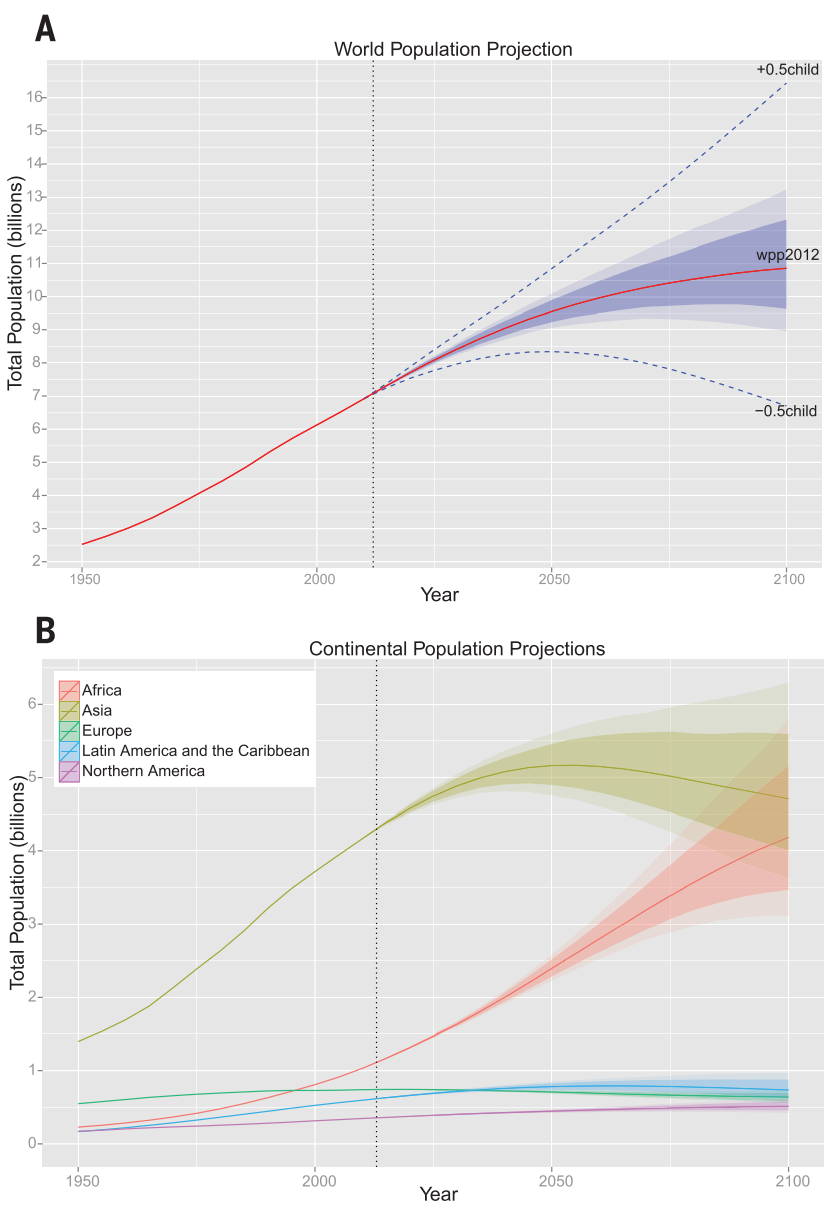
\includegraphics[scale=0.33]{./03grphs/10popul-science.png}

\begin{description}
\item[median population forecast:] increase of 4 billion to 2100, from the current 7.2 billion to 11.2 billion in 2100

\item[the largest contribution] from Sub-Saharan Africa: increase from 1 billion to 3.9 billion. 

\item[GDP is to increase 21 times:] in this area which translates into 6\% increase in CO$_2$ emissions
\end{description}
\end{multicols}
\end{center}
\end{frame}




\begin{frame}{Less than $2^{\circ}$C warming by 2100 unlikely: \textbf{results}}

\textbf{Validation of emissions predictions.}
\begin{center}
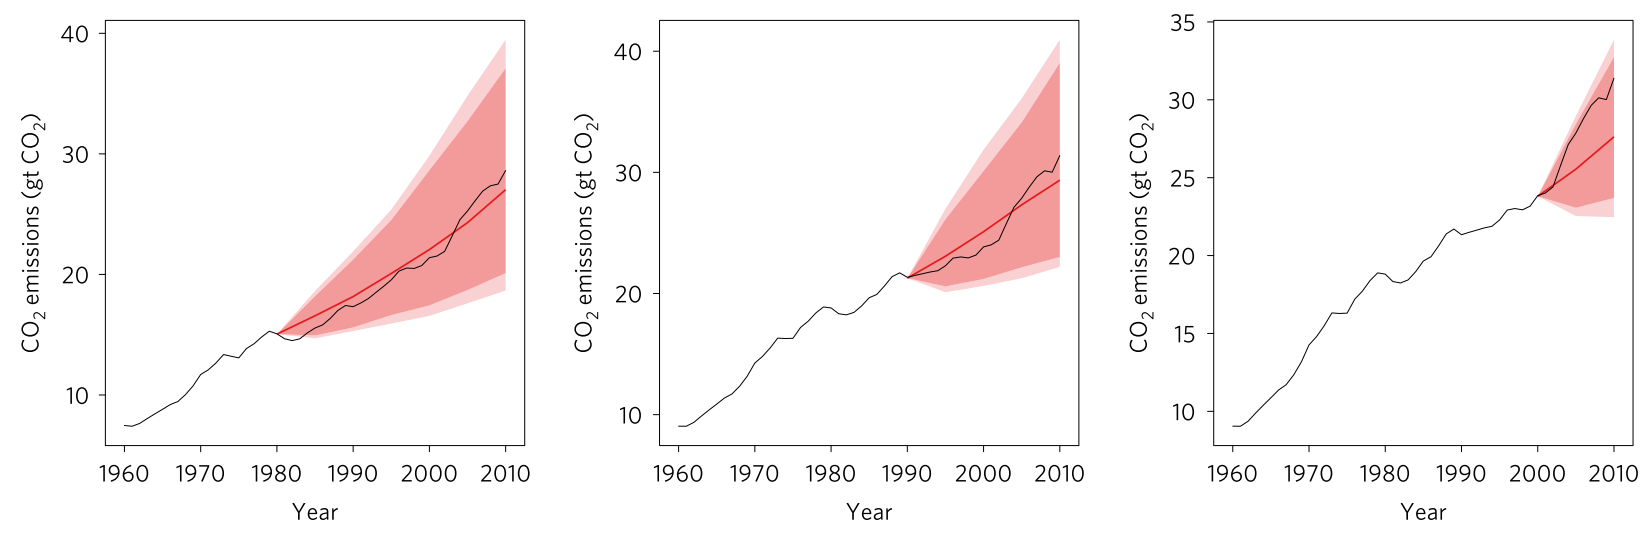
\includegraphics[scale=0.38]{./03grphs/11emissions-valid.png}
\end{center}
\begin{description}
\item[Calibrated and estimated model] assigns considerable predictive density mass to data corresponding to the forecast period in a pseudo-out-of-sample forecasting exercise

\end{description}

\end{frame}






\begin{frame}{Less than $2^{\circ}$C warming by 2100 unlikely: \textbf{results}}

\textbf{Kaya identity components predictions.}
\begin{center}
\begin{multicols}{2}
\begin{description}
\item[Decline] in intensity balanced out by the increase in GDP
\item[Population] contributes very little to emissions forecast error variance
\item[GDP] growth reduction is an unlikely policy target 
\item[Reduction in intensity] contributes a lot to emissions forecast error variance and is a feasible policy target
\end{description}

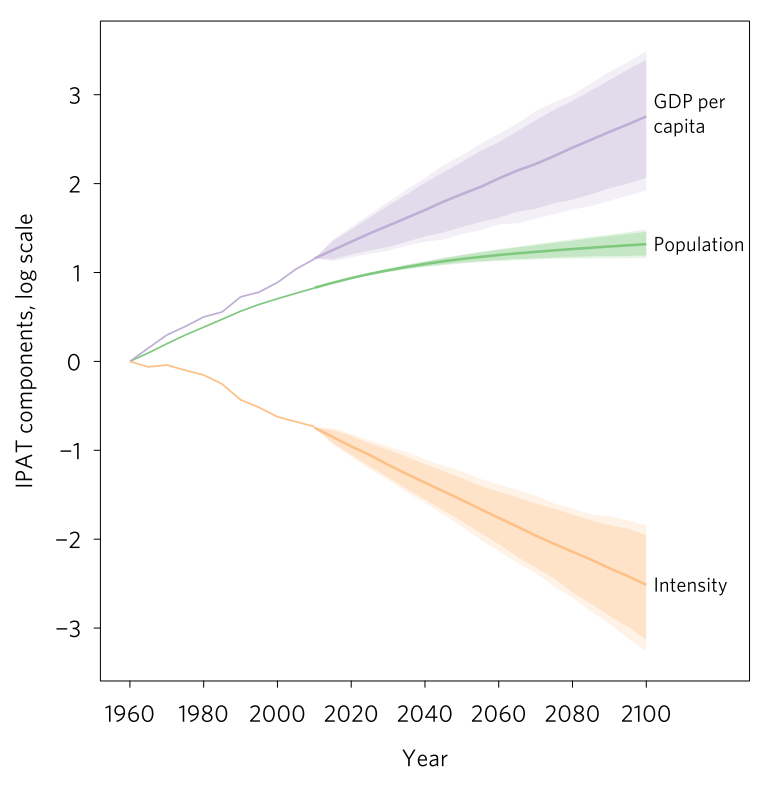
\includegraphics[scale=0.43]{./03grphs/12components.png}
\end{multicols}
\end{center}
\end{frame}






\begin{frame}{Less than $2^{\circ}$C warming by 2100 unlikely: \textbf{results}}

\textbf{CO$_2$ emissions predictions and assessment of projections.}
\begin{center}
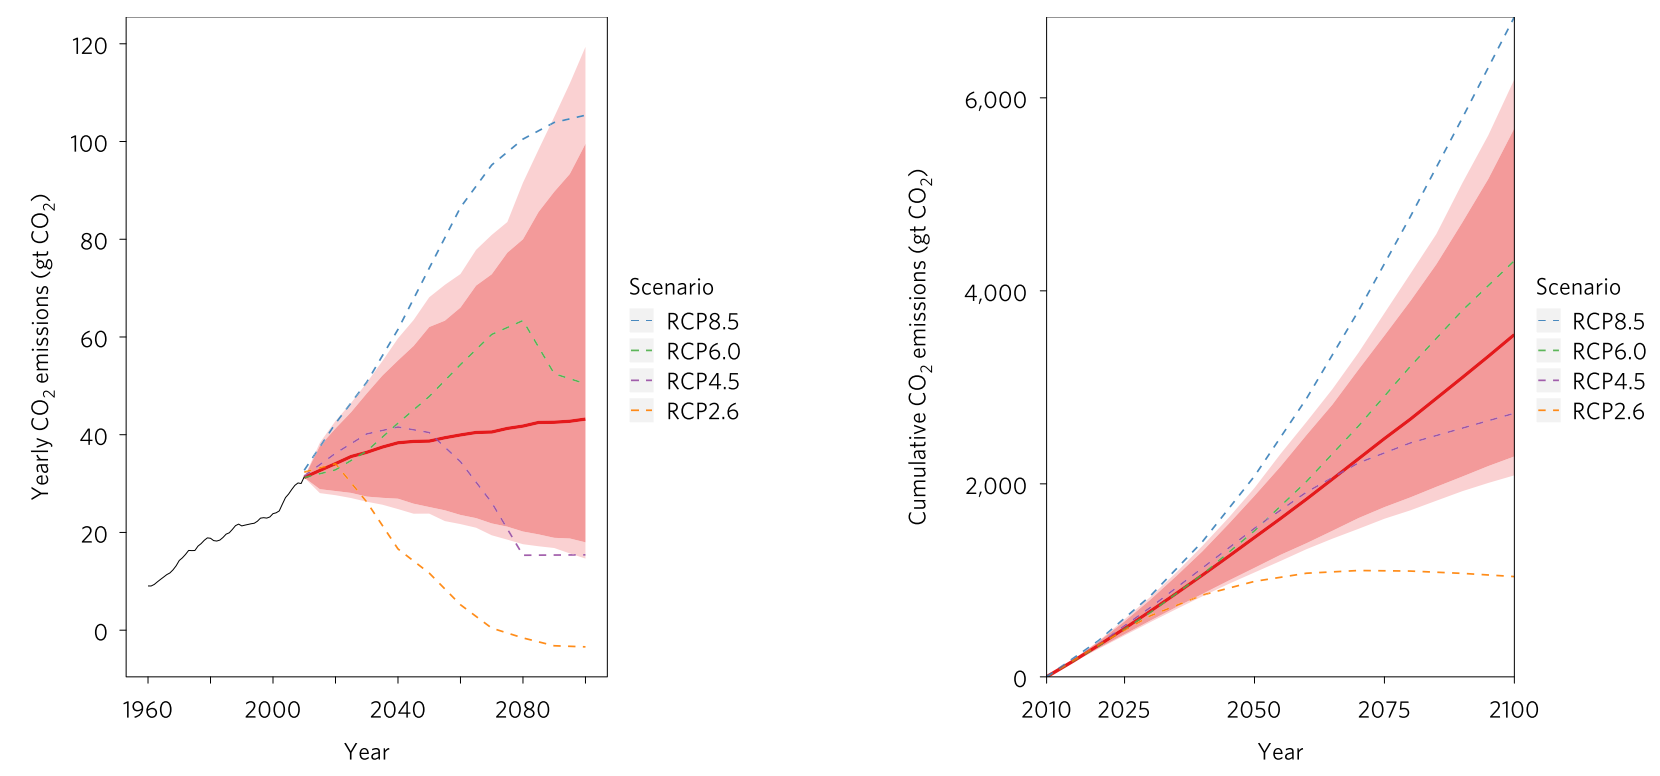
\includegraphics[scale=0.3]{./03grphs/14emissions-asses.png}
\end{center}
\begin{description}
\item[Annual emissions] are predicted to increase

\item[High- and low-level emissions scenarios] are unlikely

\item[Mid-level emissions scenarios] are confirmed with probabilistic forecasts
\end{description}

\end{frame}







\begin{frame}{Less than $2^{\circ}$C warming by 2100 unlikely: \textbf{results}}

\textbf{Predicted temperature increase.}
\begin{center}
\begin{multicols}{2}
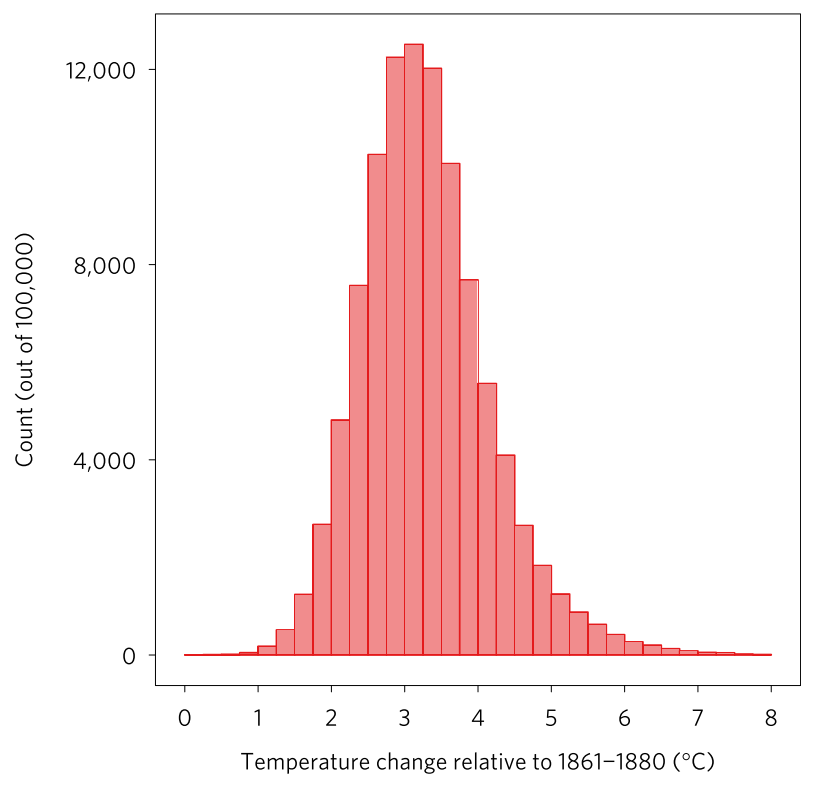
\includegraphics[scale=0.37]{./03grphs/15temp.png}

\begin{description}
\item[median increase] is equal to 3.2$^\circ$C
\item[likely range] is between 2 and 4.9$^\circ$C

\item[less than 2$^\circ$C warming] is assigned 5\% chance
\item[5\% chance] is assigned more than 4.9$^\circ$C warming

\item[less than 1.5$^\circ$C warming] is assigned 1\% chance
\end{description}
\end{multicols}
\end{center}
\end{frame}




\begin{frame}{Less than $2^{\circ}$C warming by 2100 unlikely: \textbf{results}}

\bigskip\textbf{Emissions predictions and Paris agreement.}
\begin{center}
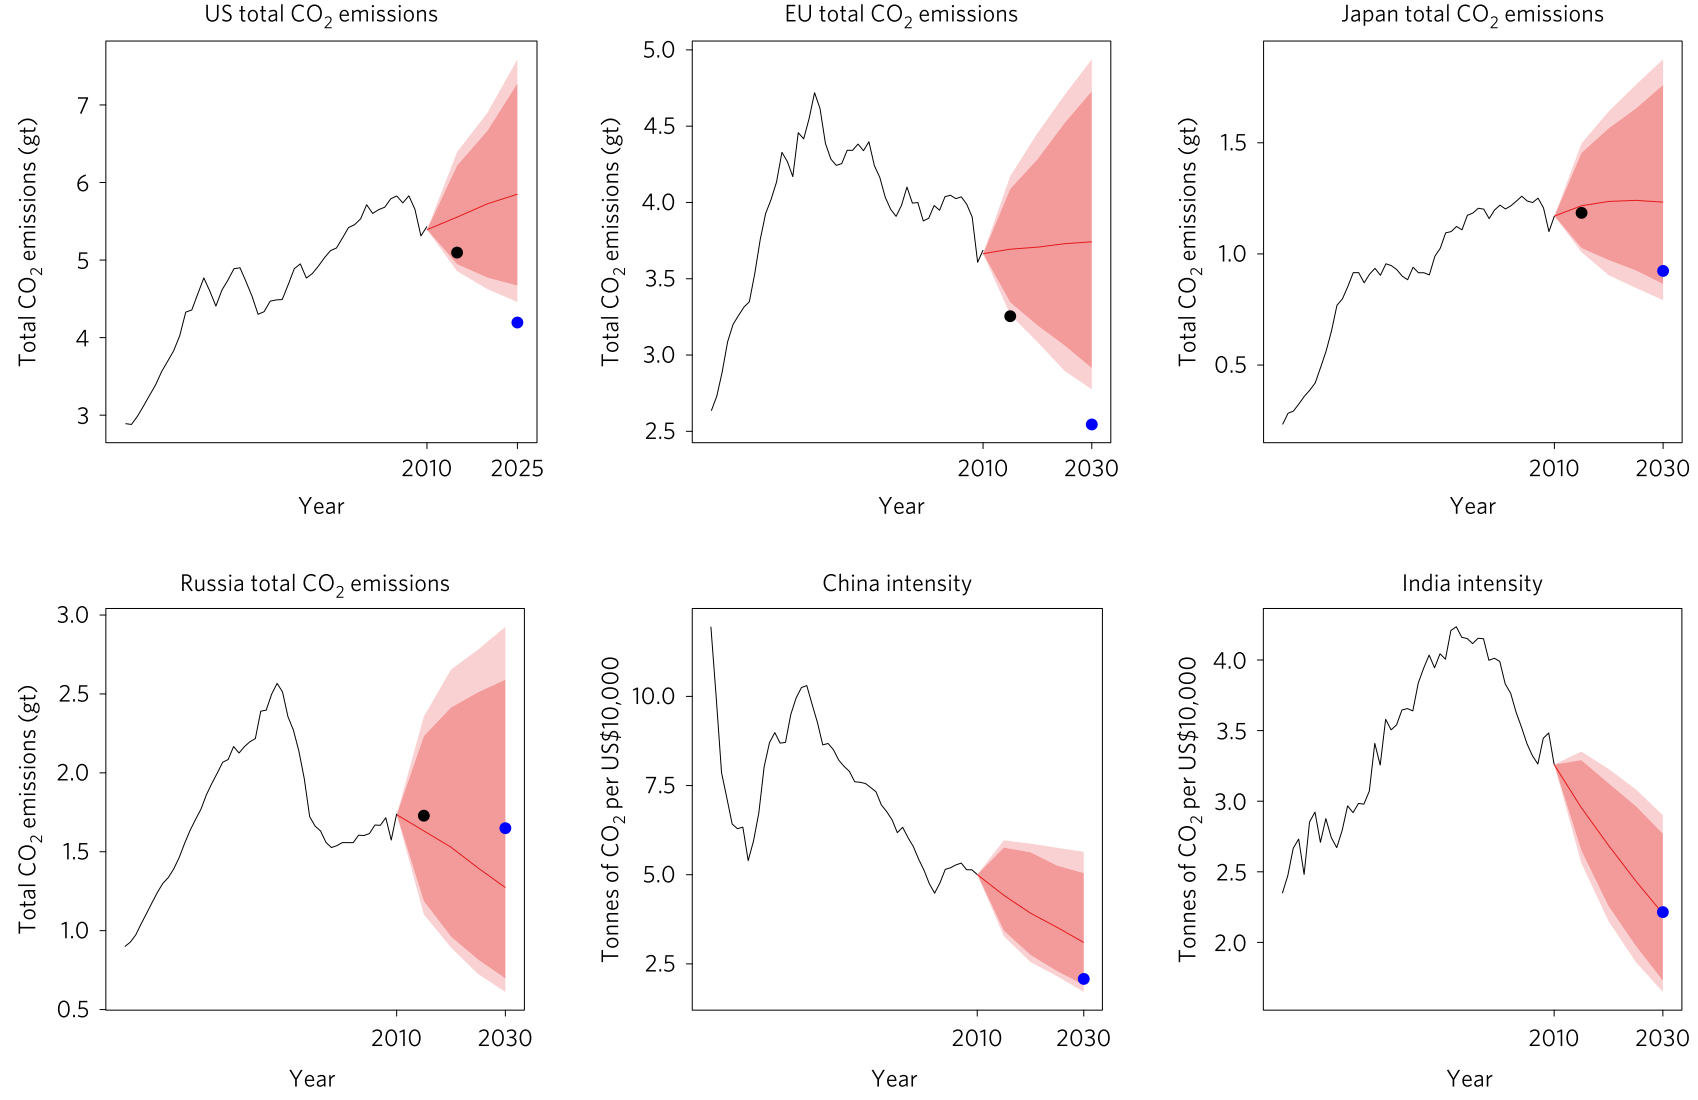
\includegraphics[scale=0.35]{./03grphs/16emissions-targets.png}

\scriptsize
{\color{black}$\bullet$ preliminary estimate 2015}, $\color{blue}\bullet$ Paris climate agreement target for 2030
\end{center}
\end{frame}













{\setbeamercolor{background canvas}{bg=gre}
\begin{frame}

\begin{adjustwidth}{-0.5cm}{0cm}
\vspace{8.3cm}\Large
\textbf{{\color{yel}Bayesian} {\color{blu}predictive model}}
\end{adjustwidth}

\end{frame}
}




\begin{frame}{Bayesian predictive model}
\textbf{Model for the frontier economy.}
\begin{center}
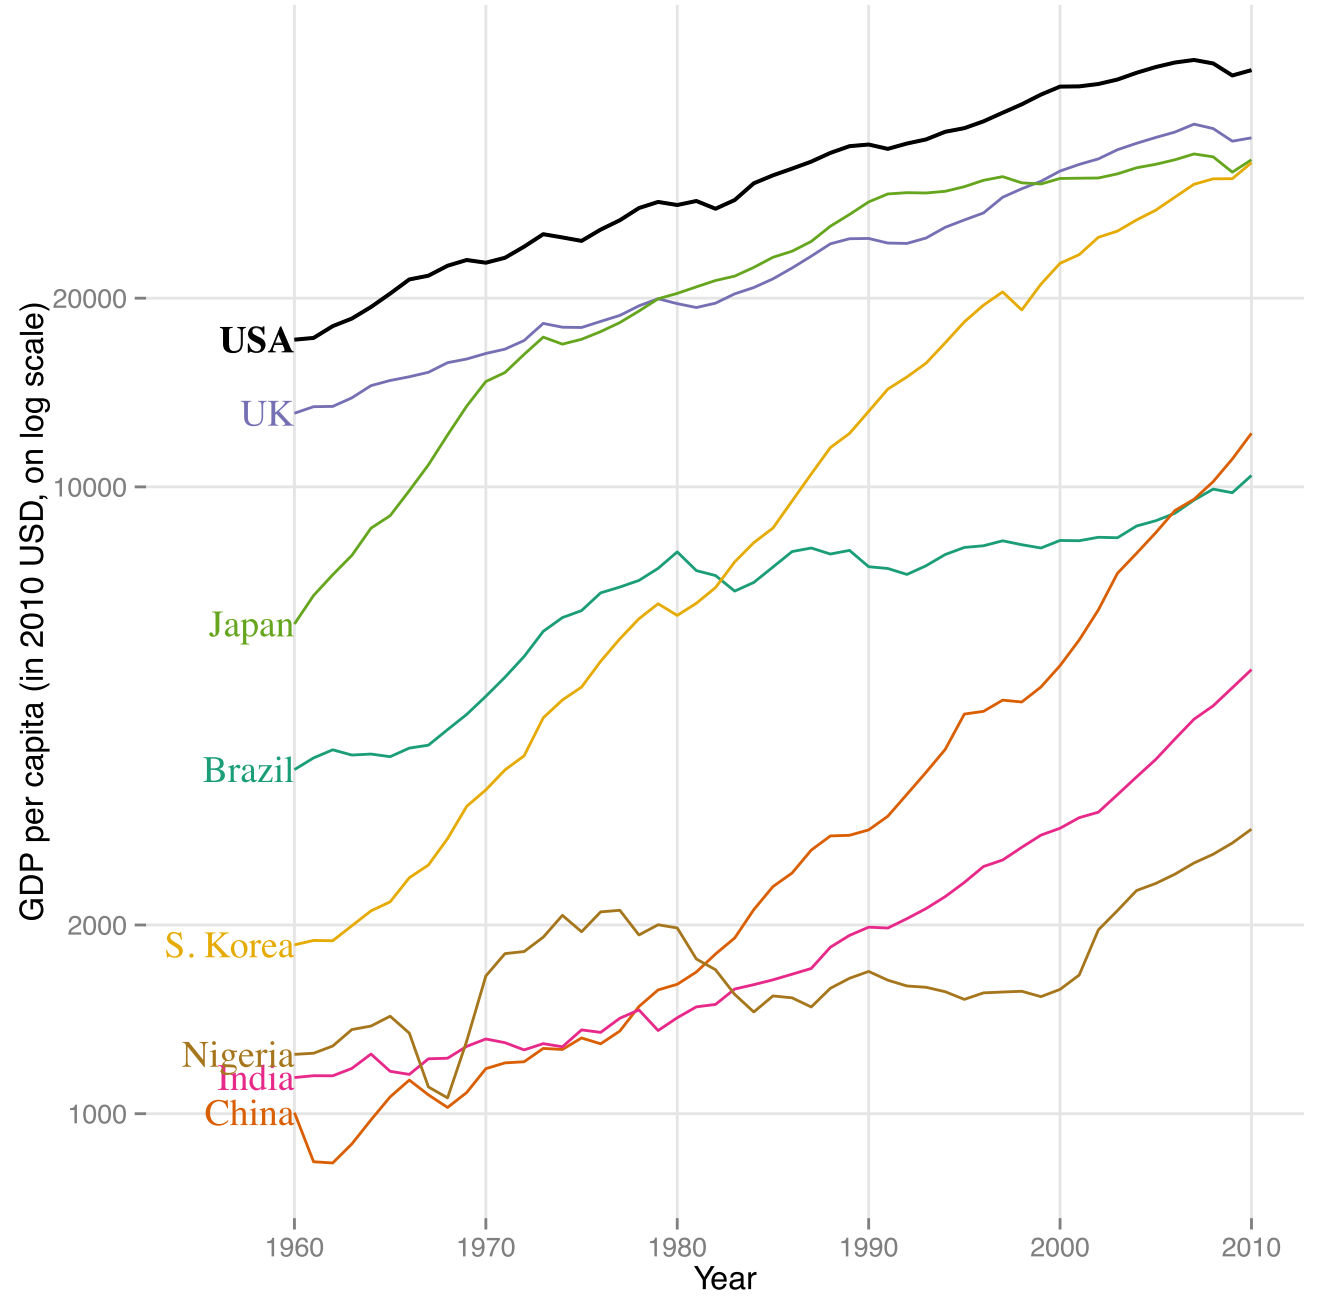
\includegraphics[scale=0.27]{./03grphs/09frontier.png}
\end{center}
\end{frame}





\begin{frame}{Bayesian predictive model}

\textbf{Model for the frontier economy.}
\begin{align*}
F_t &= F_{t-1} + \gamma +\gamma_{pre 1973}\mathcal{I}(t\leq 1973) + \epsilon_t^{(f)}\\
\epsilon_t^{(f)} &\sim\mathcal{N}\left( 0,\sigma_f^2 \right)
\end{align*}

\smallskip\begin{description}
\item[Model:] gaussian random walk with structural break in the drift

\smallskip\item[Dependent variable:] the logarithm of US annual GDP per capita

\smallskip\item[Sample period:] 1960 - 2010 ($T=50$)

\smallskip\item[Data source:] The Maddison Project: \href{http://www.ggdc.net/maddison/ maddison-project/}{www.ggdc.net/maddison/ maddison-project/}

\end{description}

\end{frame}




\begin{frame}{Bayesian predictive model}

\bigskip\textbf{Model for other economies.}
\begin{align*}
(F_t - G_{c.t}) &= \phi_c(F_{t-1}- G_{c.t-1}) + \epsilon_{c.t}^{(g)}\\
\epsilon_{c.t}^{(g)} &\sim\mathcal{N}\left( 0,\sigma_{g.c}^2 \right)\\[2ex]
\text{for } &  c=2,3,\dots,N
\end{align*}

\smallskip\begin{description}
\item[Model:] convergence to the frontier at a stationary AR(1) rate

\smallskip\item[Dependent variable:] the difference between $F_t$ and the logarithm of annual GDP data in 1990 US dollars converted to 2010 US dollars by multiplying by 1.52 based on the OECD price deflator

\smallskip\item[Sample period:] 1960 - 2010 ($T=50$)

\smallskip\item[Data source:] The Maddison Project

\end{description}

\end{frame}






\begin{frame}{Bayesian predictive model}

\textbf{Model for other economies.}
\begin{center}
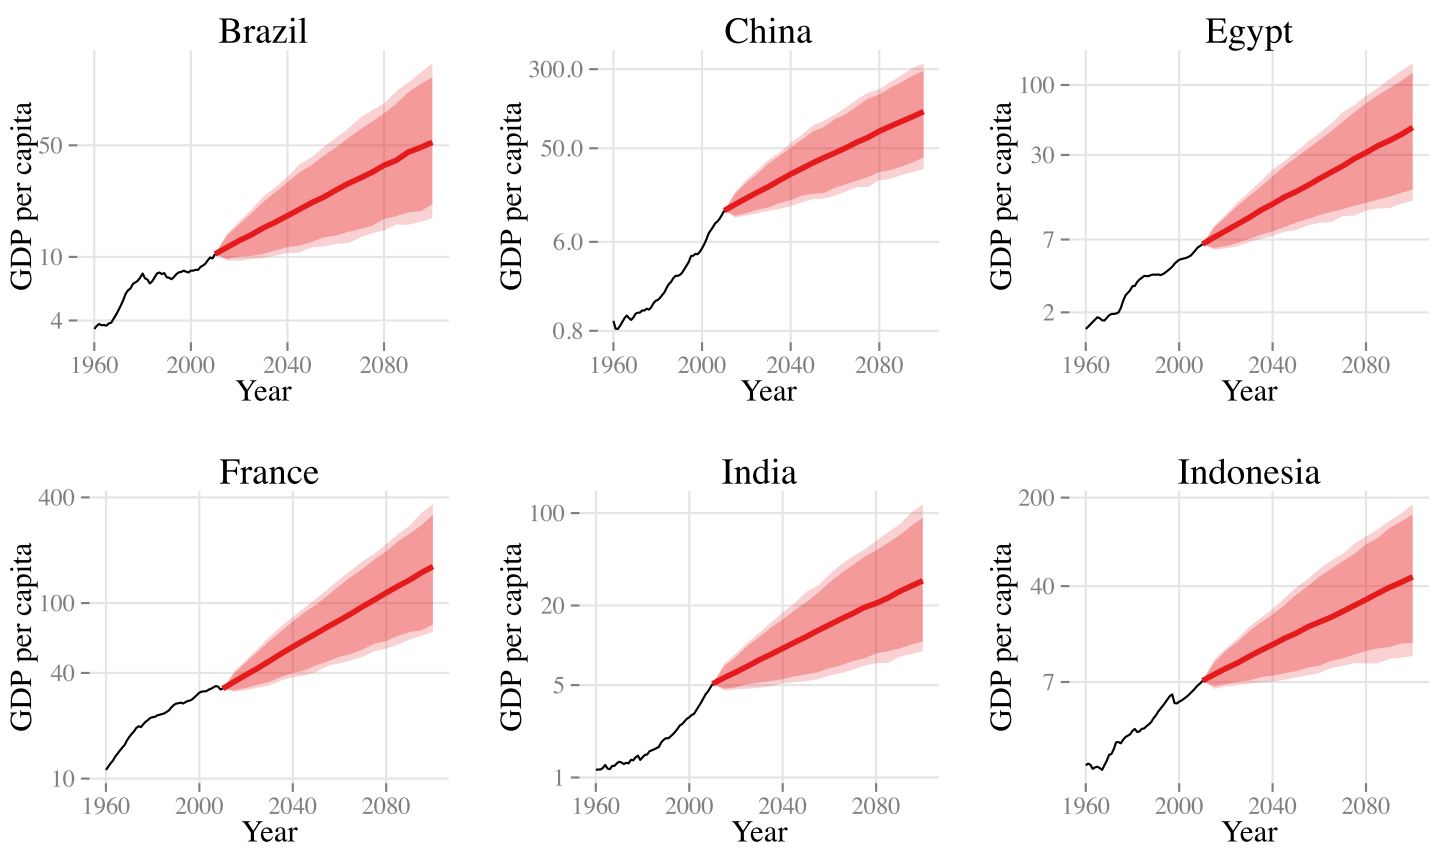
\includegraphics[scale=0.42]{./03grphs/07gdp-pred.png}
\end{center}
\end{frame}




\begin{frame}{Bayesian predictive model}

\bigskip\textbf{Carbon intensity data.}
\begin{center}
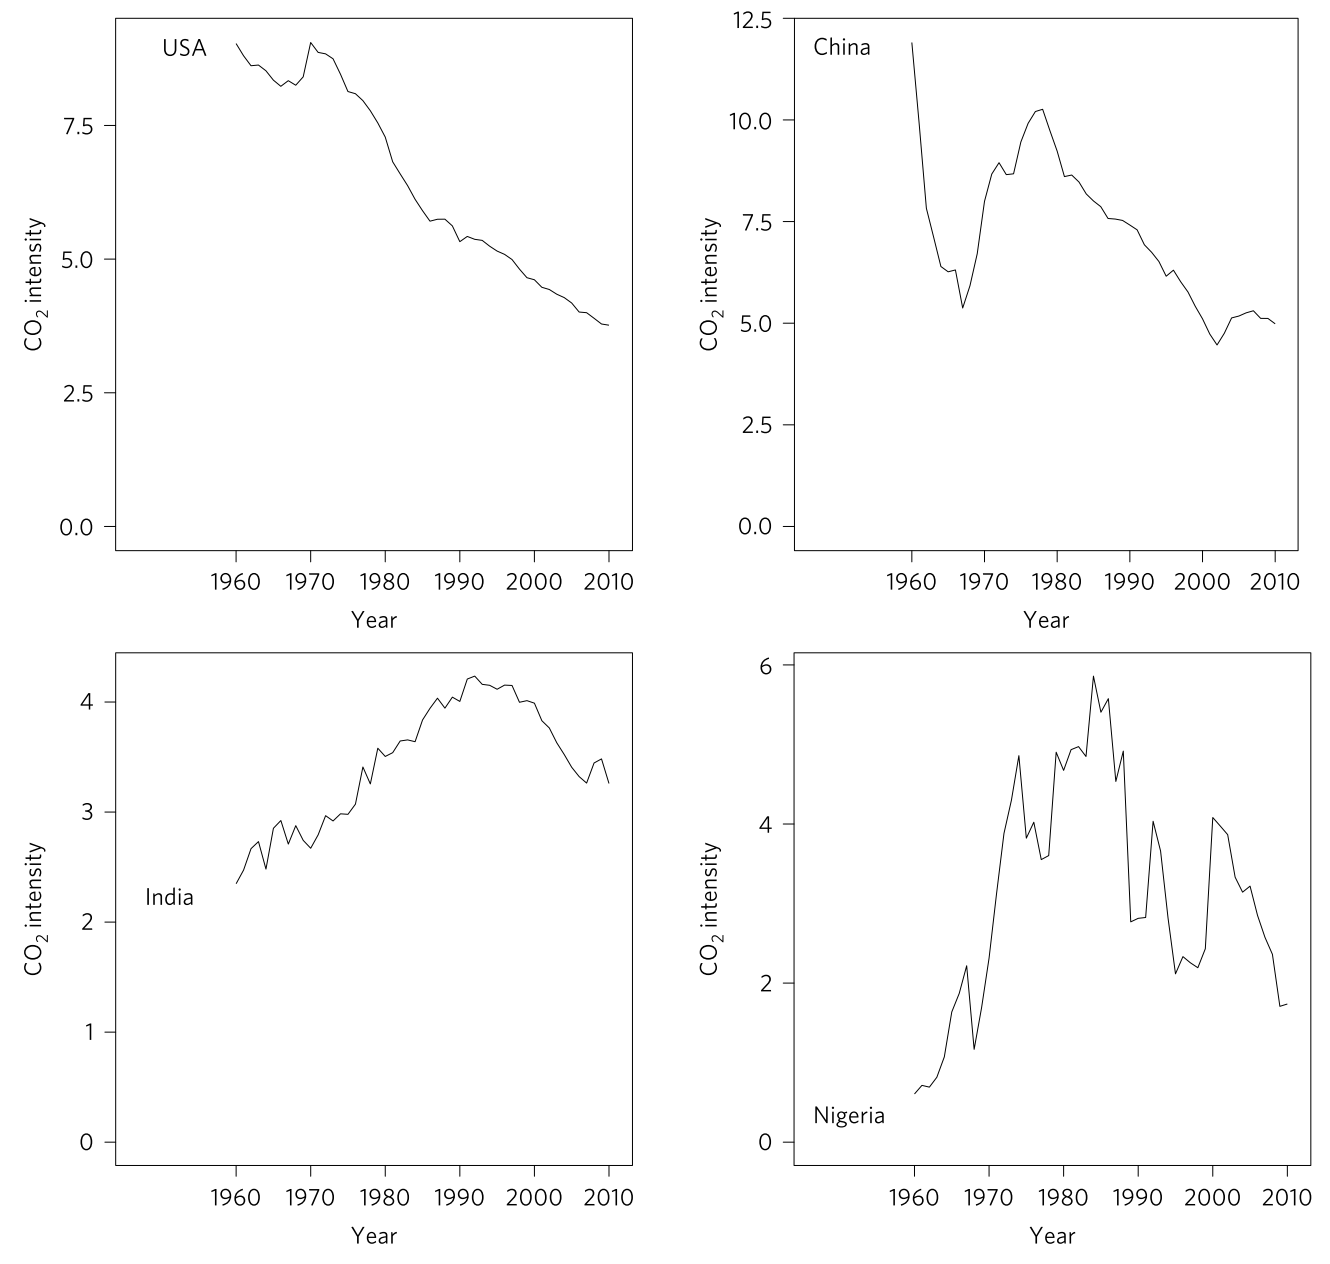
\includegraphics[scale=0.35]{./03grphs/01intensity-data.png}
\end{center}
\end{frame}



\begin{frame}{Bayesian  predictive model}

\smallskip\textbf{Model for carbon intensity.}
\begin{align*}
\tau_{c.t} &= \eta (t-\bar{t}) + \beta \tau_{c.t-1} - \delta_{c} + \epsilon_{c.t}\\
\epsilon_{c.t}|\epsilon_{c.t}^{(g)} &\sim\mathcal{N}\left( \rho\frac{\sigma_{c}}{\sigma_{g.c}},(1-\rho^2)\sigma_{c}^2 \right)
\end{align*}

\smallskip\small\begin{description}
\item[Model:] panel AR(1) model with common deterministic trend, autoregressive and correlation parameters, and country-specific fixed effects

\item[$\rho$] -- common correlation coefficient between $\epsilon_{c.t}$ and $\epsilon_{c.t}^{(g)}$

\smallskip\item[Dependent variable:] 

the logarithm of fossil fuel and cement production emissions for each country, excluding emissions from land-use change, in tonnes of CO$_2$ per US\$10,000 in 2010
Purchasing Power Parity

\item[Sample period:] post-peak series for each country -- the peak is the maximum of smoothed series using loess smoother with span 0.25

\item[Data source:] Global Carbon Budget: \href{https://www.globalcarbonproject.org/}{www.globalcarbonproject.org}

\end{description}

\end{frame}




\begin{frame}{Bayesian  predictive model}

\textbf{Model for other economies.}
\begin{center}
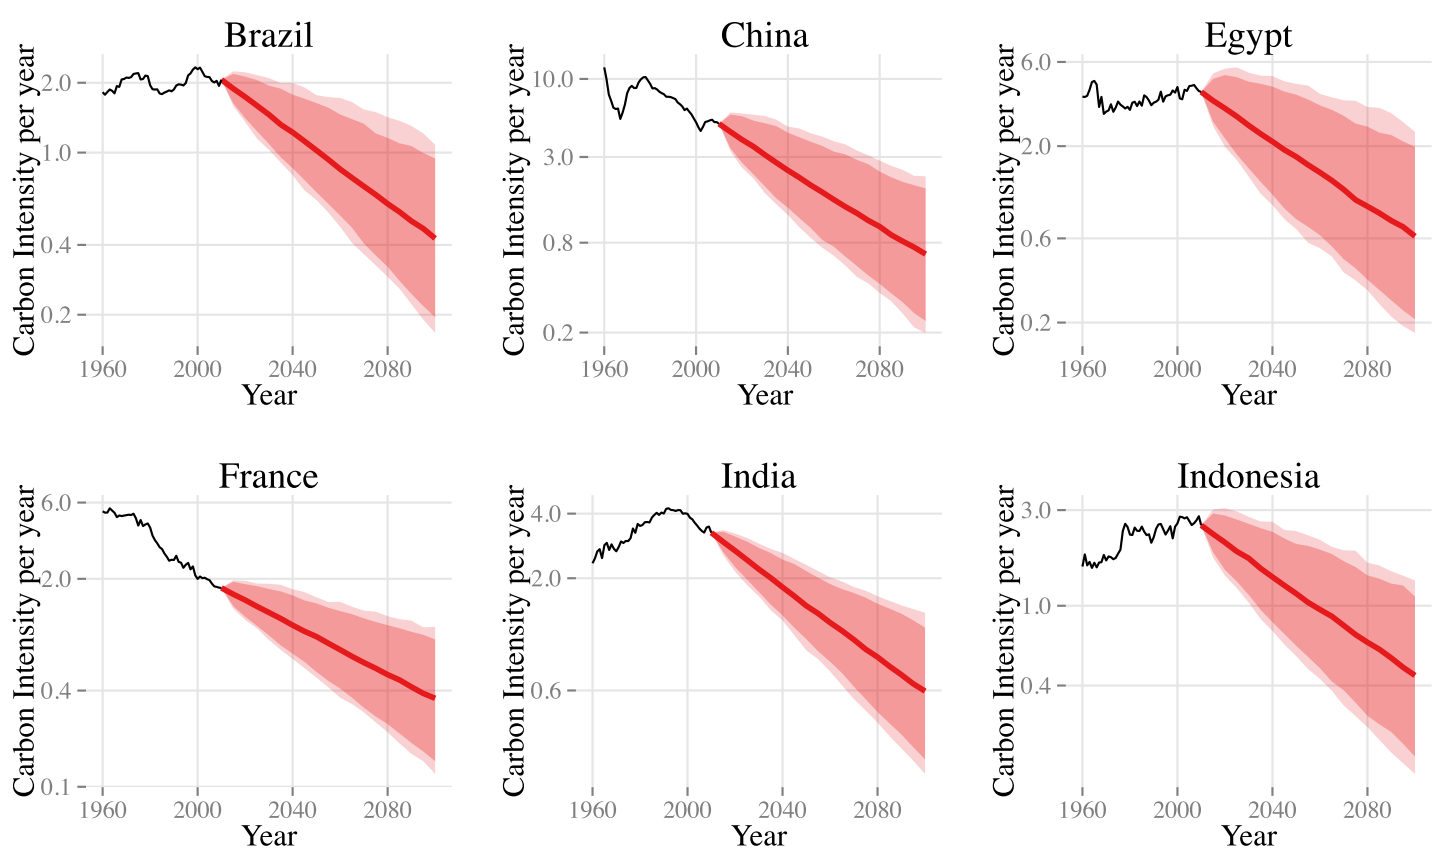
\includegraphics[scale=0.42]{./03grphs/06intensity-pred.png}
\end{center}
\end{frame}




\begin{frame}{Bayesian  predictive model}

\textbf{Joint modeling: error term specification.}\footnotesize
\begin{align*}
\begin{bmatrix} \epsilon_{t}^{(f)} \\ \epsilon_{1.t} \\ \epsilon_{2.t}^{(g)} \\ \epsilon_{2.t} \\  \vdots \\ \epsilon_{N.t}^{(g)} \\ \epsilon_{N.t} \end{bmatrix} &\sim\mathcal{N}_{2N}\left( \mathbf{0}_{2N}, 
\begin{bmatrix}
\sigma_f^2 & \rho\sigma_f\sigma_1 &0&0&\dots&0&0\\
\rho\sigma_f\sigma_1  & \sigma_1^2 &0&0&\dots&0&0\\
0&0 &\sigma_{g.2}^2 & \rho\sigma_{g.2}\sigma_2&\dots&0&0\\
0&0 & \rho\sigma_{g.2}\sigma_2 & \sigma_2^2&\dots&0&0\\
\vdots&\vdots & \vdots & \vdots&\ddots&\vdots&\vdots\\
0&0 &0&0&\dots&\sigma_{g.N}^2 & \rho\sigma_{g.N}\sigma_N\\
0&0 & 0&0&\dots&\rho\sigma_{g.M}\sigma_N & \sigma_N^2\\
\end{bmatrix} \right)
\end{align*}

\smallskip\small\begin{description}
\item[Model:] block-diagonal structure of the error term covariance matrix presuming common correlation coefficient and country-specific variances
\end{description}

\end{frame}







{\setbeamercolor{background canvas}{bg=blu}
\begin{frame}

\begin{adjustwidth}{-0.5cm}{0cm}
\vspace{8.3cm}\Large
\textbf{{\color{gre}Hierarchical} {\color{yel}prior distributions}}
\end{adjustwidth}

\end{frame}
}


\begin{frame}{Hierarchical prior distributions}

\textbf{Model for the frontier economy -- prior distributions.}
\begin{align*}
F_t &= F_{t-1} + \gamma +\gamma_{pre 1973}\mathcal{I}(t\leq 1973) + \epsilon_t^{(f)}\\
\epsilon_t^{(f)} &\sim\mathcal{N}\left( 0,\sigma_f^2 \right)\\[2ex]
\gamma &\sim\mathcal{U}[0,1]\\
\gamma_{pre 1973} &\sim\mathcal{U}[-0.1,0.1]\\
\sigma_f &\sim\log\mathcal{N}(-3,20)
\end{align*}


\end{frame}



\begin{frame}{Hierarchical prior distributions}

\textbf{Model for other economies -- prior distributions.}
\begin{align*}
(F_t - G_{c.t}) &= \phi_c(F_{t-1}- G_{c.t-1}) + \epsilon_{c.t}^{(g)}\\
\epsilon_{c.t}^{(g)} &\sim\mathcal{N}\left( 0,\sigma_{g.c}^2 \right)\\[2ex]
\phi_c|\mu_\phi, \sigma_\phi &\sim\mathcal{TN}_{[0,1]}\left(\mu_\phi, \sigma_\phi^2\right)\\
\mu_\phi &\sim\mathcal{U}[0,1] \\
\sigma_\phi &\sim \mathcal{U}[0,1]\\[2ex]
\sigma_{g.c}|\mu_g,\sigma_g &\sim\log\mathcal{N}\left(\mu_g,\sigma_g^{2}\right)\\
\mu_g &\sim\mathcal{N}\left( -6,40 \right)\\
\sigma_g & \sim \mathcal{U}[0.05,5]
\end{align*}

\end{frame}




\begin{frame}{Hierarchical prior distributions}

\bigskip\textbf{Model for carbon intensity.}\small
\begin{align*}
\tau_{c.t} &= \eta (t-\bar{t}) + \beta \tau_{c.t-1} - \delta_{c} + \epsilon_{c.t}\\
\epsilon_{c.t}|\epsilon_{c.t}^{(g)} &\sim\mathcal{N}\left( \rho\frac{\sigma_{c}}{\sigma_{g.c}},(1-\rho^2)\sigma_{c}^2 \right)\\[2ex]
\eta&\sim \mathcal{N}\left( 0.1,0.01 \right)\\
\beta&\sim \mathcal{U}[0,1]\\[1ex]
\delta_c|\mu_\delta,\sigma_\delta&\sim\mathcal{N}\left(\mu_\delta,\sigma_\delta^2\right) \\
\mu_\delta&\sim\mathcal{N}(0,1) \\
\sigma_\delta &\sim\log\mathcal{N}(-5,1.15) \\[1ex]
\sigma_{c}|\sigma_\mu,\sigma_{SD} &\sim\log\mathcal{N}\left(\sigma_\mu,\sigma_{SD}^2\right)\\
\sigma_\mu &\sim\mathcal{N}\left( -2,100 \right)\\
\sigma_{SD} & \sim \mathcal{U}[0.05,5]\\[1ex]
\rho&\sim\mathcal{U}[-1,1]
\end{align*}

\end{frame}













{\setbeamercolor{background canvas}{bg=gre}
\begin{frame}{\color{yel}Less than $2^{\circ}$C warming by 2100 unlikely}

\begin{description}
\item[Long-run forecasting] {\color{yel}of quantities that are essential for decision-makers faces multiple challenges} 

\bigskip\item[Probabilistic forecasting] {\color{yel}is crucial for realistic assessment of future tendencies } 

\bigskip\item[Hierarchical Bayesian] {\color{yel} modeling provides additional tools to calibrate the model to the objective of the research} 

\bigskip\item[Much stricter policies] {\color{yel}constraining carbon intensity of economies are required to keep the increase in global temperatures below the level triggering multiple climate change tipping points}

\end{description}

\end{frame}}


\end{document} 